\setcounter{section}{2}
\section{CÁC PHÉP TOÁN TRÊN TẬP HỢP}
\subsection{LÝ THUYẾT TRỌNG TÂM}
\subsubsection{Hợp và giao của các tập hợp}
\begin{kttrongtam}
	Cho hai tập hợp $A$ và $B$.
	\immini{Tập hợp các phần tử thuộc $A$ hoặc thuộc $B$ gọi là hợp của hai tập hợp $A$ và $B$, kí hiệu $A \cup B$.
		$$A \cup B=\{x \mid x \in A \text { hoặc } x \in B\}.$$}{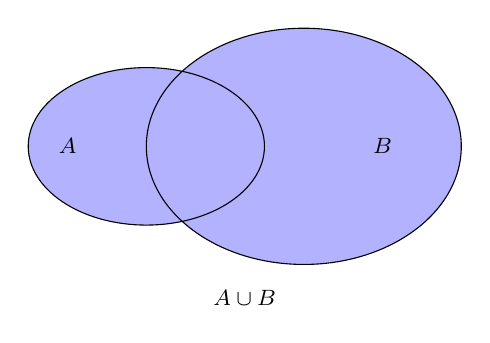
\begin{tikzpicture}[>=stealth,line join=round,line cap=round,font=\footnotesize,scale=1]
			\def\firstellipse{(0.5,0) ellipse (1.5 and 1)}
			\def\secondellipse{(2.5,0) ellipse (2 and 1.5)}
			\draw[fill=blue!30] \firstellipse \secondellipse;
			\path (current bounding box.south) node[below=2mm]{$A\cup B$};
			\node at (-0.5,0){$A$};
			\node at (3.5,0){$B$};
	\end{tikzpicture}}
	\immini{
		Tập hợp các phần tử thuộc cả hai tập hợp $A$ và $B$ gọi là giao của hai tập hợp $A$ và $B$, kí hiệu $A \cap B$.
		$$A \cap B=\{x \mid x \in A \text { và } x \in B\}.$$}{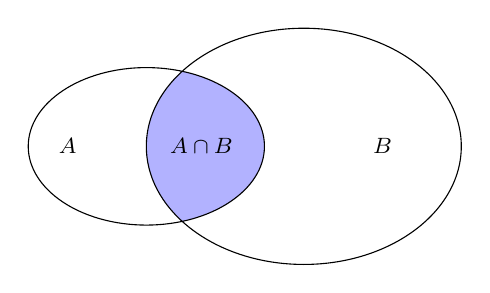
\begin{tikzpicture}[>=stealth,line join=round,line cap=round,font=\footnotesize,scale=1]
			\def\firstellipse{(0.5,0) ellipse (1.5 and 1)}
			\def\secondellipse{(2.5,0) ellipse (2 and 1.5)}
			\begin{scope}
				\clip \firstellipse;
				\fill[blue!30] \secondellipse;
			\end{scope}
			\draw \firstellipse \secondellipse;
			\node at (1.2,0){$A\cap B$};
			\node at (-0.5,0){$A$};
			\node at (3.5,0){$B$};
	\end{tikzpicture}}
\end{kttrongtam}

\begin{vd}%[0D1N3-1]
	Xác định $A \cup B$ và $A \cap B$ trong mỗi trường hợp sau:
	\begin{enumerate}
		\item $A=\{2;3;5;7\}$, $B=\{1;3;5;15\}$;
		\item $A=\{1;2;3;a;b\}$, $B=\{2;4;6;a;c;e\}$;
		\item $A$ là tập hợp các hình bình hành, $B$ là tập hợp các hình thoi.
	\end{enumerate}
	\loigiai{
		\begin{enumerate}
			\item $A \cup B=\{1;2;3;5;7;15\}$, $A \cap B=\{3;5\}$.
			\item Phương trình $x(x+2)=0$ có hai nghiệm là $0$ và $-2$, nên $A=\{-2;0\}$.\\
			Phương trình $x^{2}+2=0$ vô nghiệm, nên $B=\varnothing$.\\
			Từ đó, $A \cup B=A \cup \varnothing=A=\{-2;0\}$, $A \cap B=A \cap \varnothing=\varnothing$.
			\item Vì mỗi hình thoi cũng là hình bình hành nên $B \subset A$.\\
			Từ đó, $A \cup B=A$, $A \cap B=B$.
		\end{enumerate}
	}
\end{vd}

\begin{vd}%[0D1H3-1]
	Lớp $10$ D có $22$ bạn chơi bóng đá, $25$ bạn chơi cầu lông và $15$ bạn chơi cả hai môn thể thao này. Hỏi lớp $10$ D có bao nhiêu học sinh chơi ít nhất một trong hai môn thể thao bóng đá và cầu lông?
	\loigiai{
		\immini{Kí hiệu $A$, $B$ lần lượt là tập hợp các học sinh của lớp $10$ D chơi bóng đá, chơi cầu lông.\\
			Theo giả thiết, $n(A)=22$, $n(B)=25$, $n(A \cap B)=15$.\\
			Nhận thấy rằng, nếu tính tổng $n(A)+n(B)$ thì ta được số học sinh lớp $10$ D chơi bóng đá hoặc cầu lông, nhưng số bạn chơi cả hai môn được tính hai lần. Do đó, số bạn chơi ít nhất một trong hai môn là}{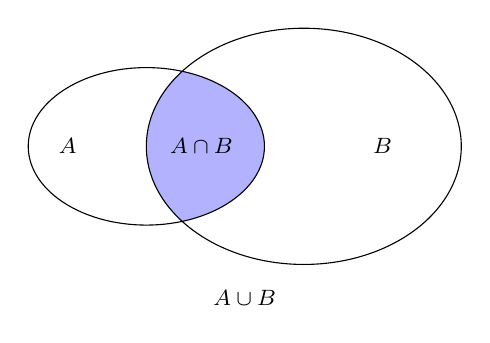
\begin{tikzpicture}[>=stealth,line join=round,line cap=round,font=\footnotesize,scale=1]
				\def\firstellipse{(0.5,0) ellipse (1.5 and 1)}
				\def\secondellipse{(2.5,0) ellipse (2 and 1.5)}
				\begin{scope}
					\clip \firstellipse;
					\fill[blue!30] \secondellipse;
				\end{scope}
				\draw \firstellipse \secondellipse;
				\node at (1.2,0){$A\cap B$};
				\node at (-0.5,0){$A$};
				\node at (3.5,0){$B$};
				\path (current bounding box.south) node[below=2mm]{$A\cup B$};
		\end{tikzpicture}}
		$$n(A \cup B)=n(A)+n(B)-n(A \cap B)=22+25-15=32.$$
		Vậy lớp $10$ D có $32$ học sinh chơi ít nhất một trong hai môn thể thao bóng đá và cầu lông.
	}
\end{vd}

\begin{nx}
	\hfill
	\begin{itemize}
		\item Nếu $A$ và $B$ là hai tập hợp hữu hạn thì $n(A \cup B)=n(A)+n(B)-n(A \cap B)$.
		\item Đặc biệt, nếu $A$ và $B$ không có phần tử chung, tức $A \cap B=\varnothing$, thì $n(A \cup B)=n(A)+n(B)$.
	\end{itemize}
\end{nx}

\subsubsection{Hiệu của hai tập hợp, phần bù của tập con}
\begin{kttrongtam}
	Cho hai tập hợp $A$ và $B$.
	\immini{Tập hợp các phần tử thuộc $A$ nhưng không thuộc $B$ gọi là hiệu của $A$ và $B$, kí hiệu $A \setminus B$.
		$$A \setminus B=\{x \mid x \in A \text { và } x \notin B\}.$$}{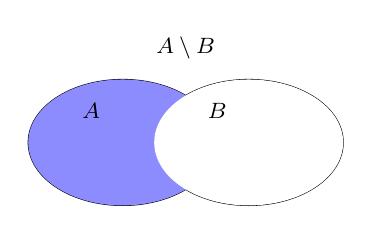
\begin{tikzpicture}[>=stealth,line join=round,line cap=round,font=\footnotesize,scale=.8]
			\draw (0.5,0) ellipse (1.5 and 1);
			\draw (2.5,0) ellipse (1.5 and 1);
			\fill[blue!45,even odd rule] (0.5,0) ellipse (1.5 and 1);
			\fill[fill=white] (2.5,0) ellipse (1.5 and 1);
			\path 
			(0,.5)coordinate[label=center:$A$](A) (2,.5)coordinate[label=center:$B$](B)
			(1.5,1.5)coordinate[label=center:$A\setminus B$](B);
	\end{tikzpicture}}
	\immini{Nếu $A$ là tập con của $E$ thì hiệu $E \setminus A$ gọi là \textbf{phần bù} của $A$ trong $E$, kí hiệu $C_{E} A$.}{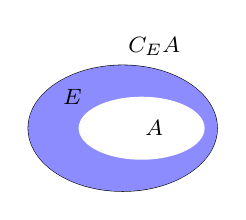
\begin{tikzpicture}[>=stealth,line join=round,line cap=round,font=\footnotesize,scale=.8]
			\draw (0.5,0) ellipse (1.5 and 1);
			\draw (.8,0) ellipse (1 and .5);
			\fill[fill=blue!45,even odd rule] (0.5,0) ellipse (1.5 and 1);
			\fill[fill=white] (.8,0) ellipse (1 and .5);
			\path 
			(-.3,.5)coordinate[label=center:$E$](S) (1,0)coordinate[label=center:$A$](A)
			(1,1.3)coordinate[label=center:$C_E A$](A);
	\end{tikzpicture}}
\end{kttrongtam}

\begin{vd}%[0D1N3-2]
	Cho $E=\{x \in \mathbb{N} \mid x<10\}$, $A=\{0;2;4;6;8\}$, $B=\{0;3;6;9\}$.
	Xác định các tập hợp $A \setminus B$, $B \setminus A$, $C_{E} A$, $C_{E} B$.
	\loigiai{
		Ta có $A \setminus B=\{2;4;8\}$, $B \setminus A=\{3;9\}$, $C_{E} A=\{1;3;5;7;9\}$, $C_{E} B=\{1;2;4;5;7;8\}$.}
\end{vd}

\begin{note}
	Trong các chương sau, để tìm các tập hợp là hợp, giao, hiệu, phần bù của những tập con của tập số thực, ta thường vẽ sơ đồ trên trục số.
\end{note}

\begin{vd}%[0D1N3-2]
	Xác định các tập hợp sau đây:
	\begin{listEX}[3]
		\item $A=[-2;1) \cup(0;3]$;
		\item $B=(-\infty;1] \cup(-2;2)$;
		\item $C=(-1;4] \cap(-3;2)$;
		\item $D=(-3;2) \setminus(1;4)$;
		\item $E=C_{\mathbb{R}}(-\infty;2)$.
	\end{listEX}
	\loigiai{
		\begin{enumerate}
			\item Để xác định tập hợp $A$, ta vẽ sơ đồ sau đây:
			\begin{center}
				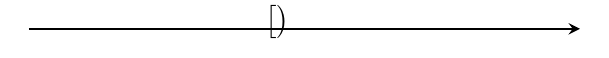
\begin{tikzpicture}[thick,>=stealth]
					\draw[->](-3,0)->(4,0);
					\IntervalLR{-3}{-2}
					\def\skipInterval{0.5cm}
					\IntervalGRF{}{}{\big[}{-2}
					\IntervalLR{1}{3.8}
					\def\skipInterval{0.5cm}
					\IntervalGRF{\big)}{1}{}{}
				\end{tikzpicture}\\
				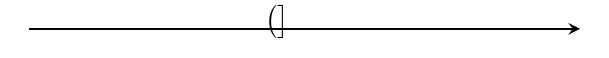
\begin{tikzpicture}[thick,>=stealth]
					\draw[->](-3,0)->(4,0);
					\IntervalLR{-3}{0}
					\def\skipInterval{0.5cm}
					\IntervalGRF{}{}{\big(}{0}
					\IntervalLR{3}{3.8}
					\def\skipInterval{0.5cm}
					\IntervalGRF{\big]}{3}{}{}
				\end{tikzpicture}\\
				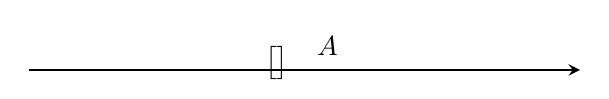
\begin{tikzpicture}[thick,>=stealth]
					\draw[->](-3,0)->(4,0);
					\IntervalLR{-3}{-2}
					\def\skipInterval{0.5cm}
					\IntervalGRF{}{}{\big[}{-2}
					\IntervalLR{3}{3.8}
					\def\skipInterval{0.5cm}
					\IntervalGRF{\big]}{3}{}{}
					\path (0.5,0.3)coordinate[label=center:$A$](A);
				\end{tikzpicture}
			\end{center}
			Từ sơ đồ, ta thấy $A=[-2;3]$.
			\item Để xác định tập hợp $B$, ta vẽ sơ đồ sau đây:
			\begin{center}
				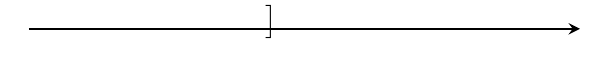
\begin{tikzpicture}[thick,>=stealth]
					\draw[->](-3,0)->(4,0);
					\IntervalLR{1}{3.8}
					\def\skipInterval{0.5cm}
					\IntervalGRF{\big]}{1}{}{}
				\end{tikzpicture}\\
				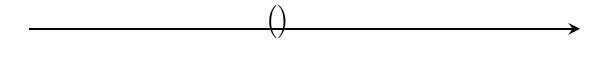
\begin{tikzpicture}[thick,>=stealth]
					\draw[->](-3,0)->(4,0);
					\IntervalLR{-3}{-2}
					\def\skipInterval{0.5cm}
					\IntervalGRF{}{}{\big(}{-2}
					\IntervalLR{2}{3.8}
					\def\skipInterval{0.5cm}
					\IntervalGRF{\big)}{2}{}{}
				\end{tikzpicture}\\
				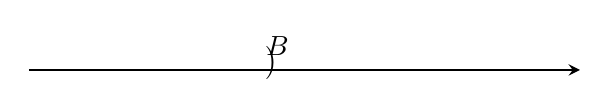
\begin{tikzpicture}[thick,>=stealth]
					\draw[->](-3,0)->(4,0);
					\IntervalLR{2}{3.8}
					\def\skipInterval{0.5cm}
					\IntervalGRF{\big)}{2}{}{}
					\path (0,0.3)coordinate[label=center:$B$](B);
				\end{tikzpicture}
			\end{center}
			Từ sơ đồ, ta thấy $B=(-\infty;2)$.
			\item Để xác định tập hợp $C$, ta vẽ sơ đồ sau đây:
			\begin{center}
				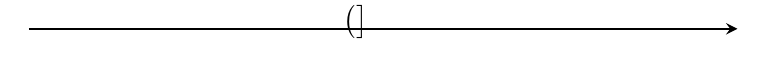
\begin{tikzpicture}[thick,>=stealth]
					\draw[->](-4,0)->(5,0);
					\IntervalLR{-4}{-1}
					\def\skipInterval{0.5cm}
					\IntervalGRF{}{}{\big(}{-1}
					\IntervalLR{4}{4.8}
					\def\skipInterval{0.5cm}
					\IntervalGRF{\big]}{4}{}{}
				\end{tikzpicture}\\
				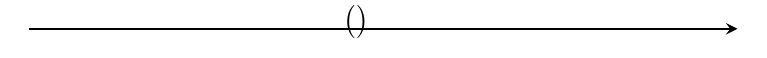
\begin{tikzpicture}[thick,>=stealth]
					\draw[->](-4,0)->(5,0);
					\IntervalLR{-4}{-3}
					\def\skipInterval{0.5cm}
					\IntervalGRF{}{}{\big(}{-3}
					\IntervalLR{2}{4.8}
					\def\skipInterval{0.5cm}
					\IntervalGRF{\big)}{2}{}{}
				\end{tikzpicture}\\
				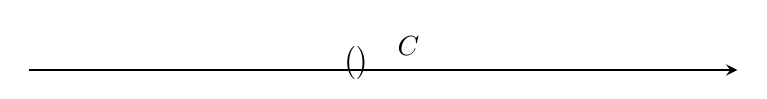
\begin{tikzpicture}[thick,>=stealth]
					\draw[->](-4,0)->(5,0);
					\IntervalLR{-4}{-1}
					\def\skipInterval{0.5cm}
					\IntervalGRF{}{}{\big(}{-1}
					\IntervalLR{2}{4.8}
					\def\skipInterval{0.5cm}
					\IntervalGRF{\big)}{2}{}{}
					\path (0.5,0.3)coordinate[label=center:$C$](C);
				\end{tikzpicture}
			\end{center}
			Từ sơ đồ, ta thấy $C=(-1;2)$.
			\item Để xác định tập hợp $D$, ta vẽ sơ đồ sau đây:
			\begin{center}
				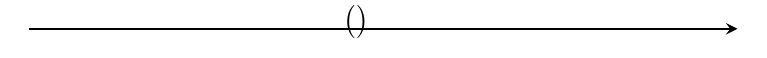
\begin{tikzpicture}[thick,>=stealth]
					\draw[->](-4,0)->(5,0);
					\IntervalLR{-4}{-3}
					\def\skipInterval{0.5cm}
					\IntervalGRF{}{}{\big(}{-3}
					\IntervalLR{2}{4.8}
					\def\skipInterval{0.5cm}
					\IntervalGRF{\big)}{2}{}{}
				\end{tikzpicture}\\
				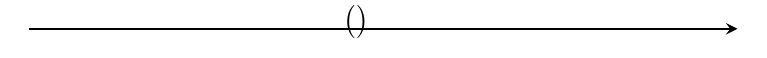
\begin{tikzpicture}[thick,>=stealth]
					\draw[->](-4,0)->(5,0);
					\IntervalLR{-4}{1}
					\def\skipInterval{0.5cm}
					\IntervalGRF{}{}{\big(}{1}
					\IntervalLR{4}{4.8}
					\def\skipInterval{0.5cm}
					\IntervalGRF{\big)}{4}{}{}
				\end{tikzpicture}\\
				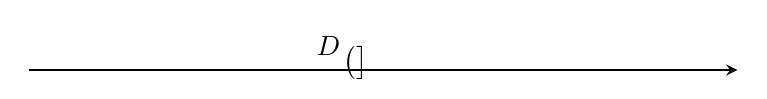
\begin{tikzpicture}[thick,>=stealth]
					\draw[->](-4,0)->(5,0);
					\IntervalLR{-4}{-3}
					\def\skipInterval{0.5cm}
					\IntervalGRF{}{}{\big(}{-3}
					\IntervalLR{1}{4.8}
					\def\skipInterval{0.5cm}
					\IntervalGRF{\big]}{1}{}{}
					\path (-0.5,0.3)coordinate[label=center:$D$](D);
				\end{tikzpicture}
			\end{center}
			Từ sơ đồ, ta thấy $D=(-3;1]$.
			\item Để xác định tập hợp $E$, ta vẽ sơ đồ sau đây:
			\begin{center}
				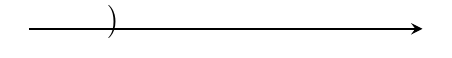
\begin{tikzpicture}[thick,>=stealth]
					\draw[->](-1,0)->(4,0);
					\IntervalLR{2}{3.8}
					\def\skipInterval{0.5cm}
					\IntervalGRF{\big)}{2}{}{}
				\end{tikzpicture}\\
				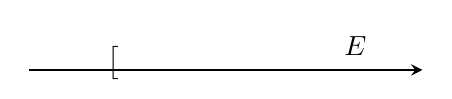
\begin{tikzpicture}[thick,>=stealth]
					\draw[->](-1,0)->(4,0);
					\IntervalLR{-1}{2}
					\def\skipInterval{0.5cm}
					\IntervalGRF{}{}{\big[}{2}
					\path (3,0.3)coordinate[label=center:$E$](E);
				\end{tikzpicture}
			\end{center}
			Từ sơ đồ, ta thấy $E=[2;+\infty)$.
		\end{enumerate}
	}
\end{vd}
\subsection{BÀI TẬP RÈN LUYỆN}
\caulc
\begin{ex}%[0D1N3-1]%Câu 1-NB
	Cho hai tập hợp $A=\{-1;2;3;5;7\}$, $B=\{1;2;3;4;5\}$. Khi đó giao của hai tập hợp là
	\choice
	{\True $A\cap B=\{2;3;5\}$}
	{$A\cap B=\{-1;2;3;4;5;7\}$}
	{$A\cap B=\{-1\}$}
	{$A\cap B=\{7\}$}
	\loigiai{
		Ta có $A\cap B=\{2;3;5\}$.}
\end{ex}
\begin{ex}%[0D1N3-1]%Câu 2-NB
	Cho hai tập hợp ${A=\{1;2;3;4;5;6;7\}}$, $B=\{5;6;7;8\}$ Tìm tập $C=A\cup B$
	\choice
	{\True $C=\{1;2;3;4;5;6;7;8\}$}
	{$C=\{1;2;3;4;8\}$}
	{$C=\{5;6;7\}$}
	{$C=\{1;2;3;4\}$}
	\loigiai{
		Ta có $C=\{1;2;3;4;5;6;7;8\}$}
\end{ex}
\begin{ex}%[0D1N3-3]%Câu 3-NB
	Tập hợp $[-5;1)\cup (0;4]$ bằng tập hợp nào sau đây?
	\choice
	{$(0;1)$}
	{$[0;1]$}
	{\True $[-5;4]$}
	{$[-5;0]$}
	\loigiai{
		Ta có $[-5;1)\cup (0;4]=[-5;4]$}
\end{ex}
\begin{ex}%[0D1N3-1]%Câu 4-NB
	Cho hai tập hợp $A=\{-7;0;5;7\},B=\{-3;5;7;13\}$. Khi đó tập $A\cap B$ là
	\choice
	{\True $\{5;7\}$}
	{$\{-7;-3;0;5;7;13\}$}
	{$\{-7;0\}$}
	{$\{13\}$}
	\loigiai{
		Ta tìm phần chung của cả hai tập hợp.}
\end{ex}
\begin{ex}%[0D1N3-1]%Câu 5-NB
	Cho $A=\{0;1;2\}$, $B=\{-1;0;1\}$. Khi đó $A\cap B$ là
	\choice
	{$\{-1\}$}
	{$\{2\}$}
	{\True $\{0;1\}$}
	{$\{-1;0;1;2\}$}
	\loigiai{
		Ta có $A\cap B=\{0;1\}$.}
\end{ex}
\begin{ex}%[0D1N3-1]%Câu 6-NB
	Cho $A=\{1;5\};B=\{1;3;5\}$. Chọn kết quả đúng trong các kết quả sau
	\choice
	{$A\cap B=\{1\}$}
	{$A\cap B=\{1;3\}$}
	{\True $A\cap B=\{1;5\}$}
	{$A\cap B=\{1;3;5\}$}
	\loigiai{
		$A=\{1;5\};B=\{1;3;5\}$.\\
		Suy ra $A\cap B=\{1;5\}$.}
\end{ex}
\begin{ex}%[0D1N3-3]%Câu 7-NB
	Tập hợp $X=(-\infty;2]\cap (-6;+\infty)$ là
	\choice
	{$[-6;2]$}
	{\True $(-6;2]$}
	{$(-4;9]$}
	{$\mathbb{R}$}
	\loigiai{
		Ta có $X=(-6;2]$.}
\end{ex}
\begin{ex}%[0D1N3-3]%Câu 8-NB
	Cho tập hợp $A=[3;8)$, $B=(-\infty;4)$. Tìm $A\cap B$
	\choice
	{$(3;4)$}
	{\True $[3;4)$}
	{$(4;8)$}
	{$(-\infty;8)$}
	\loigiai{
		$A\cap B=[3;4)$.}
\end{ex}
\begin{ex}%[0D1N3-3]%Câu 9-NB
	Cho tập hợp $X=(-\infty;2]\cap (-6;+\infty)$. Khẳng định nào sau đây là đúng?
	\choice
	{\True $X=(-6;2]$}
	{$(-6;+\infty)$}
	{$X=(-\infty;+\infty)$}
	{$X=(-\infty;2]$}
	\loigiai{
		Ta có $X=(-\infty;2]\cap (-6;+\infty)=(-6;2]$.}
\end{ex}
\begin{ex}%[0D1N3-2]%Câu 10-NB
	Cho $A\subset B$. Khẳng định nào sau đây là đúng?
	\choice
	{$\mathrm{C}_B A=\{x\in B|\,x\in A\}$}
	{\True $\mathrm{C}_B A=\{x\in B|\,x\notin A\}$}
	{$\mathrm{C}_B A=\{x\notin B|\,x\notin A\}$}
	{$\mathrm{C}_B A=\{x\notin B|\,x\in A\}$}
	\loigiai{
		Theo định nghĩa, đáp áp đúng là $\mathrm{C}_B A=\{x\in B|\,x\notin A\}$.
	}
\end{ex}
\begin{ex}%[0D1N3-2]%Câu 11-TH
	Cho hai tập hợp $A=\left\{x\in \mathbb{N}|-5\le 2x-\dfrac{1}{3}\le 3\right\},\,B=\{x\in \mathbb{Z}|3x+10>1\}$. Khẳng định nào sau đây là đúng?
	\choice
	{$\mathrm{C}_B A=\{2;3;4;\ldots\}$}
	{$\mathrm{C}_B A=\{-3;-2;-1;2;3;4;\ldots\}$}
	{$\mathrm{C}_B A=\{0;1;2;3;4;\ldots\}$}
	{\True $\mathrm{C}_B A=\{-2;-1;2;3;4;\ldots\}$}
	\loigiai{
		Ta có 
		\begin{eqnarray*}
			A&=&\{x\in \mathbb{N}|-5\le 2x-\dfrac{1}{3}\le 3\} \Rightarrow A =\{0;1\}.\\
			B&=&\{x\in \mathbb{Z}|\,3x+10>1\} \Rightarrow B =\{-2;-1;0;1;2;3;\ldots\}.
		\end{eqnarray*}
		Dễ thấy $A\subset B \Rightarrow \mathrm{C}_B A=\{-2;-1;2;3;4;\ldots\}$.
	}
\end{ex}
\begin{ex}%[0D1N3-2]%Câu 12-TH
	Cho hai tập hợp $A=\{x\in \mathbb{N}| 2x-9\le 0 .\}$, $B=\{x\in \mathbb{Z}| 2x^2-3x+1=0 .\}$. Xác định $B\setminus A$.
	\choice
	{$\{1\}$}
	{$\{0;2;3;4\}$}
	{\True $\varnothing $}
	{$\{\varnothing\}$}
	\loigiai{
		Ta có $2x-9\le 0\Leftrightarrow x\le \dfrac{9}{2}$, do $x\in \mathbb{N}$ nên $A=\{0;1;2;3;4\}$.\\
		Lại có $2x^2-3x+1=0\Leftrightarrow \hoac{& x=\dfrac{1}{2}\notin \mathbb{Z} \\ & x=1\in \mathbb{Z}}$ nên $B=\{1\}$.\\
		Do đó $B\setminus A=\varnothing $.
	}
\end{ex}
\cauds
\begin{ex}%[0D1N3-1]%Câu 1-NB
	Cho các tập hợp $A=\{-3;-2;-1;0;1;2;3\}$; $B=\{0;1;4;5\}$; $C=\{-4;-3;1;2;5;6\}$.
	\choiceTF
	{\True $A\cup B=\{-3;-2;-1;0;1;2;3;4;5\}$}
	{$A\cap B=\{0\}$}
	{\True $(A\cup B)\cap C=\{-3;1;2;5\}$}
	{\True $A\cap B\cap C=\{1\}$}
	\loigiai{
		\begin{itemchoice}
			\itemch $A\cup B=\{-3;-2;-1;0;1;2;3;4;5\}$.
			\itemch $A\cap B=\{0;1\}$.
			\itemch $(A\cup B)\cap C=\{-3;1;2;5\}$.
			\itemch $A\cap B\cap C=\{1\}$
		\end{itemchoice}
	}
\end{ex}
\begin{ex}%[0D1H3-5]
	Lớp 10A có $19$ học sinh giỏi Toán, $16$ học sinh giỏi Lý, $16$ học sinh giỏi Hoá, $10$ học sinh giỏi cả Toán và Lý, $11$ học sinh giỏi cả Toán và Hoá, $8$ học sinh giỏi cả Lý và Hoá, $7$ học sinh giỏi cả ba môn Toán, Lý, Hoá. Khi đó
	\choiceTF
	{Số học sinh giỏi đúng hai môn Hoá và Lý là $8$ học sinh}
	{\True Số học sinh giỏi đúng hai môn Hoá và Toán là $4$ học sinh}
	{\True Số học sinh giỏi đúng hai môn Toán và Lý là $3$ học sinh}
	{\True Số học sinh giỏi đúng một môn là $14$ học sinh}
	\loigiai{
		Gọi $T$; $L$; $H$ lần lượt là tập hợp các học sinh giỏi môn Toán, Lý, Hóa.\\
		Vẽ biểu đồ Ven và tính số phần tử từng tập hợp ta được như hình vẽ
		\begin{center}
			\begin{tikzpicture}[scale=0.7,font=\footnotesize,line join=round,line cap=round,>=stealth]
				\path
				(0,0) coordinate (A)
				(2,0) coordinate (B)
				(1,-1.8) coordinate (C)
				;		
				\node at ($(A)+(120:1.4)$){$T$};
				\node at ($(B)+(60:1.4)$){$L$};
				\node at ($(C)+(-90:1.4)$){$H$};
				\node at ($(A)+(150:1)$){$5$}; %Chỉ Giỏi T
				\node at ($(B)+(40:0.5)$){$5$}; %Chỉ Giỏi L
				\node at ($(C)+(-90:0.6)$){$4$}; %Chỉ Giỏi H
				\node at ($(A)+(20:1.2)$){$3$}; %Giỏi T và L
				\node at ($(A)+(-20:1.2)$){$7$}; %Giỏi cả ba môn
				\node at ($(A)+(-87:1.1)$){$4$}; %Giỏi T và H
				\node at ($(A)+(-30:2.3)$){$1$}; %Giỏi L và H
				\draw (C) circle(1.8cm) (B) circle(1.8cm) (A) circle(1.8cm);			
			\end{tikzpicture}
		\end{center}
		Khi đó
		\begin{itemchoice}
			\itemch Số học sinh giỏi đúng hai môn Hoá và Lý là $8-7=1$ học sinh.
			\itemch Số học sinh giỏi đúng hai môn Hoá và Toán là $11-7=4$ học sinh.
			\itemch Số học sinh giỏi đúng hai môn Toán và Lý là $10-7=3$ học sinh.
			\itemch Số học sinh giỏi đúng một môn là $5+5+4=14$ học sinh.
		\end{itemchoice}
	}
\end{ex}
\caukq
\begin{ex}%[0D1N3-1]%Câu 1-NB
	Cho hai tập hợp $A=(-3;3)$ và $B=(0;+\infty)$. Biết $A\cup B=(a;+\infty)$. Tìm $a$.
	\shortans[]{-3}
	\loigiai{
				\begin{center}
			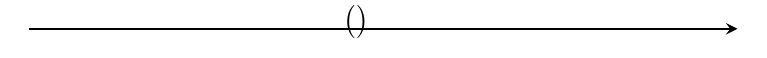
\begin{tikzpicture}[thick,>=stealth]
				\draw[->](-4,0)->(5,0);
				\IntervalLR{-4}{-3}
				\def\skipInterval{0.5cm}
				\IntervalGRF{}{}{\big(}{-3}
				\IntervalLR{2}{4.8}
				\def\skipInterval{0.5cm}
				\IntervalGRF{\big)}{3}{}{}
			\end{tikzpicture}\\
			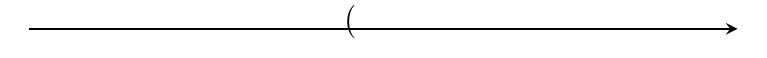
\begin{tikzpicture}[thick,>=stealth]
				\draw[->](-4,0)->(5,0);
				\IntervalLR{-4}{1}
				
				\IntervalGRF{}{}{\big(}{0}
				
			\end{tikzpicture}\\
			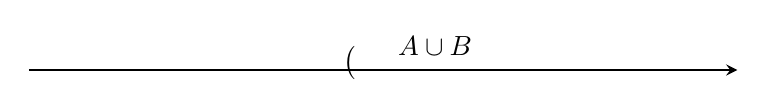
\begin{tikzpicture}[thick,>=stealth]
				\draw[->](-4,0)->(5,0);
				\IntervalLR{-4}{-3}
				\def\skipInterval{0.5cm}
				\IntervalGRF{}{}{\big(}{-3}
				
				\path (1,0.3)coordinate[label=center:$A\cup B$](D);
			\end{tikzpicture}
		\end{center}
		Ta có $A \cup B=(-3;+\infty)$.\\
		Vậy $a=-3$.
	}
\end{ex}

\begin{ex}%[0D1H3-3]%Câu 2-TH
	Cho hai tập hợp $A=\{x \in \mathbb{R}\mid-5 \leq x<1\}$; $B=\{x \in \mathbb{R}\mid-3<x \leq 3\}$. Biết $A \cap B=(a;b)$, $a<b$. Tính $a+b$.
	
	\shortans[]{-2}
	\loigiai{
		Ta có $A=[-5;1)$, $B=(-3;3]$.\\
				\begin{center}
			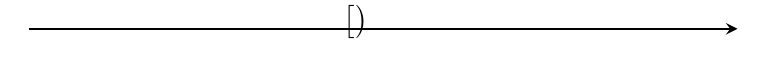
\begin{tikzpicture}[thick,>=stealth]
				\draw[->](-4,0)->(5,0);
				\IntervalLR{-4}{-1}
				\def\skipInterval{0.5cm}
				\IntervalGRF{}{}{\big[}{-5}
				\IntervalLR{4}{4.8}
				\def\skipInterval{0.5cm}
				\IntervalGRF{\big)}{1}{}{}
			\end{tikzpicture}\\
			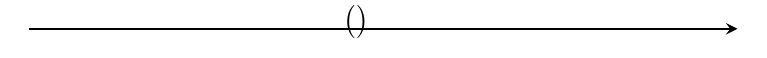
\begin{tikzpicture}[thick,>=stealth]
				\draw[->](-4,0)->(5,0);
				\IntervalLR{-4}{-3}
				\def\skipInterval{0.5cm}
				\IntervalGRF{}{}{\big(}{-3}
				\IntervalLR{2}{4.8}
				\def\skipInterval{0.5cm}
				\IntervalGRF{\big)}{3}{}{}
			\end{tikzpicture}\\
			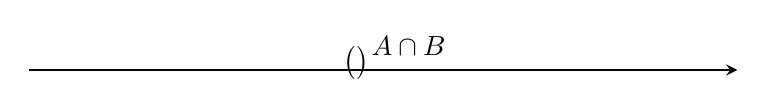
\begin{tikzpicture}[thick,>=stealth]
				\draw[->](-4,0)->(5,0);
				\IntervalLR{-4}{-1}
				\def\skipInterval{0.5cm}
				\IntervalGRF{}{}{\big(}{-3}
				\IntervalLR{2}{4.8}
				\def\skipInterval{0.5cm}
				\IntervalGRF{\big)}{1}{}{}
				\path (0.5,0.3)coordinate[label=center:$A\cap B$](C);
			\end{tikzpicture}
		\end{center}
		$\Rightarrow A \cap B=(-3;1)$.\\
		Suy ra $a=-3$; $b=1$.\\
		Vậy $a+b=-2$.
	}
\end{ex}
\begin{ex}%[0D1H3-5]%Câu 4-TH
	Kết quả điểm trung bình môn lớp $11$B$_1$ có $15$ học sinh giỏi Văn, $22$ học sinh giỏi Toán. Tìm số học sinh giỏi ít nhất một trong hai môn Toán và Văn biết lớp $11$B$_1$ có $40$ học sinh, và có $14$ học sinh không đạt học sinh giỏi một trong hai môn Toán hoặc Văn. 
	
	\shortans[]{26}
	\loigiai{
		Số học sinh học giỏi ít nhất một trong hai môn Toán và Văn là $40-14=26$.
		}
\end{ex}
\begin{ex}%[0D1H3-5]%Câu 5-TH
	Lớp $10$B$_1$ có $7$ học sinh giỏi Toán, $5$ học sinh giỏi Lý, $6$ học sinh giỏi Hóa, $3$ học sinh giỏi cả Toán và Lý, $4$ học sinh giỏi cả Toán và Hóa, $2$ học sinh giỏi cả Lý và Hóa, $1$ học sinh giỏi cả $3$ môn Toán, Lý, Hóa được minh họa bằng biểu đồ Ven dưới đây. Tính số học sinh giỏi ít nhất một môn (Toán, Lý, Hóa) của lớp $10$B$_1$.
	\begin{center}
		\begin{tikzpicture}[scale=0.9,font=\footnotesize,line join=round,line cap=round,>=stealth]
			\path
			(0,0) coordinate (A)
			(2,0) coordinate (B)
			(1,-1.8) coordinate (C)
			;		
			\node at ($(A)+(150:1)$){$1$};
			\node at ($(B)+(40:0.5)$){$1$};
			\node at ($(C)+(-90:0.6)$){$1$};
			\node at ($(A)+(20:1.2)$){$2$};
			\node at ($(A)+(-25:1.2)$){$1$};
			\node at ($(A)+(-87:1.1)$){$3$};
			\node at ($(A)+(-30:2.3)$){$1$};
			\draw (C) circle(1.8cm) (B) circle(1.8cm) (A) circle(1.8cm);	
			\draw[->] (100:2.8)node[above]{Toán}--($(A)+(100:1.8)$);
			\draw[->] ($(B)+(60:2.8)$)node[right]{Lý}--($(B)+(60:1.8)$);
			\draw[->] ($(C)+(-50:2.5)$)node[right]{Hóa}--($(C)+(-50:1.8)$);	
			\draw[->] ($(A)+(70:3.5)$)node[above]{Giỏi Toán Lý}--($(A)+(-30:0.8)$);
			\draw[->] ($(A)+(70:3.5)$)--($(A)+(24:1.4)$);
			\draw[->] ($(C)+(0:4)$)node[right]{Giỏi Lý Hóa}--($(A)+(-30:1.4)$);
			\draw[->] ($(C)+(0:4)$)--($(A)+(-30:2.7)$);
			\draw[->] ($(C)+(200:4)$)node[below]{Giỏi Toán Hóa}--($(A)+(-80:1.4)$);
			\draw[->] ($(C)+(200:4)$)--($(A)+(-35:2.7)$);
		\end{tikzpicture}
	\end{center}
	
	\shortans[]{10}
	\loigiai{
		Nhìn vào biểu đồ, số học sinh giỏi ít nhất $1$ trong $3$ môn là $1+2+1+3+1+1+1=10$.
	}
\end{ex}
\cautl
\begin{bt}%[0D1N3-1]%Câu 1-NB
	Cho hai tập hợp $A=\{-7;0;5;7\}$, $B=\{-3;5;7;13\}$. Tìm $A\cap B$, $A\cup B$, $A\setminus B$, $B\setminus A$.
	\loigiai{
	\begin{itemize}
		\item $A\cap B=\{5;7\}$.
		\item $A\cup B=\{-7;-3;0;5;7;13\}$.
		\item $A\setminus B=\{-7;0\}$.
		\item $B\setminus A=\{-3;13\}$.
	\end{itemize}}
\end{bt}

\begin{bt}%[0D1N3-2]%Câu 4-NB
	Cho các tập hợp $X$; $Z$; $W$ như hình vẽ.
	\begin{center}
		\begin{tikzpicture}[scale=1,font=\footnotesize,line join=round,line cap=round,>=stealth]
			\path
			(0,0) coordinate (A)
			(2,0) coordinate (B)			
			;		
			\node at ($(A)+(110:1)$){$1$};
			\node at ($(A)+(150:1)$){$10$};
			\node at ($(A)+(190:1)$){$4$};
			\node at ($(A)+(230:1)$){$5$};
			\node at ($(A)+(65:0.85)$){$6$};
			\node at ($(A)+(-65:0.85)$){$9$};
			\node at ($(A)+(20:1.15)$){$2$};
			\node at ($(A)+(-20:1.15)$){$7$};
			\node at ($(A)+(0:2.3)$){$3$};	
			\node at ($(A)+(50:2.3)$){$8$};	
			\draw (A) circle(1.5cm) (B) circle(2cm) (B) circle(1.6cm);	
			\draw ($(A)+(90:1.5)$)node[above]{$W$}
			($(B)+(40:2)$)node[right]{$X$}
			($(B)+(-90:1.55)$)node[below]{$Z$};						
		\end{tikzpicture}
	\end{center}
	Tìm tập hợp $W\cap X$ và $W\cap X\setminus Z$.
	\loigiai{
		Ta có $W\cap X=\{6;9;2;7\}$.\\
		$W\cap X\setminus Z=(W\cap X)\setminus Z=\{6;9\}$.}
\end{bt}
\begin{bt}%[0D1V3-5]%Câu 10-VD
	Kết quả điểm trung bình môn lớp $11$B$_1$ có $15$ học sinh giỏi Văn, $22$ học sinh giỏi Toán. Tìm số học sinh giỏi cả Văn và Toán biết lớp $11$B$_1$ có $40$ học sinh, và có $14$ học sinh không đạt học sinh giỏi một trong hai môn Toán hoặc Văn.
	\loigiai{
		\begin{center}
			\begin{tikzpicture}[scale=0.8,font=\footnotesize,line join=round,line cap=round,>=stealth]			
				\path
				(0,0) coordinate (A)
				(2,-0.3) coordinate (B)
				;
				\draw ($(A)+(200:1.8)$)--(200:2.5)node[left]{\fbox{Toán}}
				($(B)+(-30:1.5)$)--($(B)+(-30:2)$)node[right]{\fbox{Văn}};				
				\draw (A) circle(1.8cm) (B) circle(1.5cm);			
				\node at (-0.5,-0.3){$22$};
				\node at (1.22,-0.3){?};
				\node at (2.4,-0.2){$15$};
			\end{tikzpicture}
		\end{center}
		Số học sinh học giỏi ít nhất một trong hai môn Toán và Văn là $40-14=26$.\\
		Số học sinh chỉ giỏi Toán mà không giỏi Văn (Phần Toán sau khi bỏ đi phần giao).\\
		là $26-15=11$.\\
		Vậy số học sinh giỏi cả hai môn Toán và Văn (Phần giao nhau) là $22-11=11$.\\
		\textbf{Cách 2.}
		Số học sinh học giỏi ít nhất một trong hai môn Toán và Văn là $40-14=26$.\\
		Số học sinh giỏi cả hai môn Toán và Văn là $22+15-26=11$.}
\end{bt}

